\clearpage
\section{Absorptionskoeffizient}

\subsection{Linearer Absorptionskoeffizient}

Zur Bestimmung des Massenabsorptionskoeffizienten vom Aluminium, Eisen und Blei stellen wir jeweils 
unterschiedlich dicke/viele Stücke Abschirmmaterial zwischen Probe und Detektor. Als Präperat verwendet man  Dann misst man jeweils das Spektrum und und 
integrierte die Counts dann über die Spektrallinie hinweg auf. Dabei werde immer mindestens 1000 Counts unter dem Integral abgewartet, 
um ein Signal-Rausch-Verhältnis von über 10 aufgrund der Poisson-Statistik zu erhalten. \\
Zuerst messen wir dabei immer ohne Abschirmmaterial, aber mit Abstandshalter. In diesen legen wir dann das Abschirmmaterial und messen dieses aus. 
Dabei nehmen wir mehr Messwerte bei dünner Abschirmdicke $d$, da diese beim numerischen Bestimmen der Parameter vorteilhafter sind. \\
Gemessen wurde in der Reihenfolge Aluminium, Eisen, Blei und als Integralgrenzen wurden die Töpfe 442 und 451 verwendet.

Die Intensität der Gammastrahlung verhält sich dabei in Abhängigkeit der Dicke wie folgt:

\begin{equation}
    I = I_0 \exp(- \mu d) +I_R
    \label{Intensitaet}
\end{equation}

$I_0$ = Intensität vor Absorber, $I_R$ = Intensität des Rauschens, $\mu$ = linearer Absorptionskoeffizient, $d$ = Absorberdicke. 

Aus dem obigen Integral und der gemessenen Zeit kann man dann eine Zählrate ermitteln. Diese ist direkt proportional zur Intensität. 
Aus dieser und den Absorberdicken kann man dann numerisch mit der Methode der kleinsten Quadrate die optimalen Parameter bestimmen. Außerdem kann man 
noch den Fehler durch das schätzen des Parameters schätzen.\\

\subsubsection*{Aluminium}

Für Alu ergibt sich folgender Verlauf wie in Abbildung \ref{AbsorbtionkoeffAlu} zu sehen.\\

\begin{figure}[ht]
    \centering
    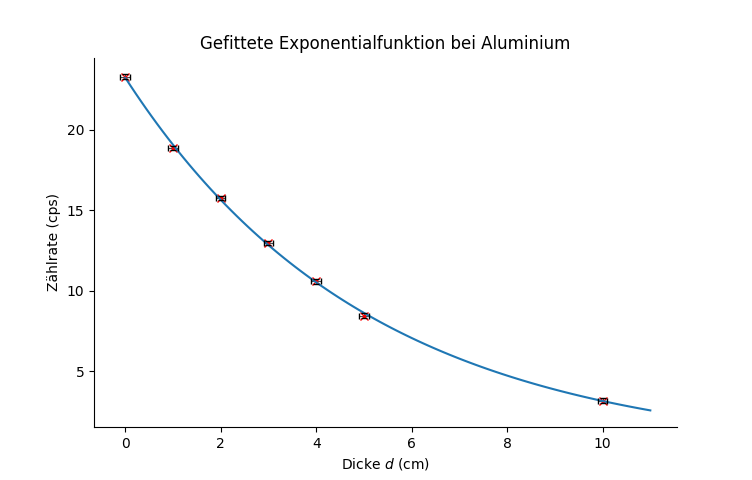
\includegraphics[width = \linewidth]{Bilder/Auswertung/AbsorbtioskAlu.png}
    \caption{Zählrate bei jeweiliger Absorberdicke $d$}
    \label{AbsorbtionkoeffAlu}
\end{figure}

Dabei muss beachtet werden, dass der oben beschrieben Fehler nicht den realen Fehler wiederspiegelt, da er noch nicht die Unsicherheiten der Messung beinhaltet. 
Sie enthält diese aber schon zu einem großen Teil, da die Unsicherheit der Messung auch den - unter einem bestimmten Signifikanzniveau möglichen - Parameterberich für $\mu$ 
vergrößert.

\begin{center}
    \centering
    \textcolor{red}{$\mu_{Alu}= (0,196 \pm 0,014) \mathrm{cm}^{-1}$}
\end{center}

Da die Fehlerbalken der Punkte so klein sind, werden diese bei den folgenden Grafiken weggelassen, da diese nur als Vertrauensstütze in das vorrausgesetzte Modell dienen. Dabei kann man sich 
immer wieder überzeugen, dass dieses den Sachverhalt sehr gut beschreibt.

\subsubsection*{Eisen}
Bei Eisen wird wie oben vorgegangen. Dabei ergibt sich folgender Kurvenverlauf (Abbildung \ref{AbsorbtionkoeffFe}). Dabei ist schon am Graphen eindeutig eine stärkere Abschirmung zu sehen. Diese spiegelt sich dementsprechend 
auch in dem linearen Absorptionskoeffizient wieder.

\begin{figure}[ht]
    \centering
    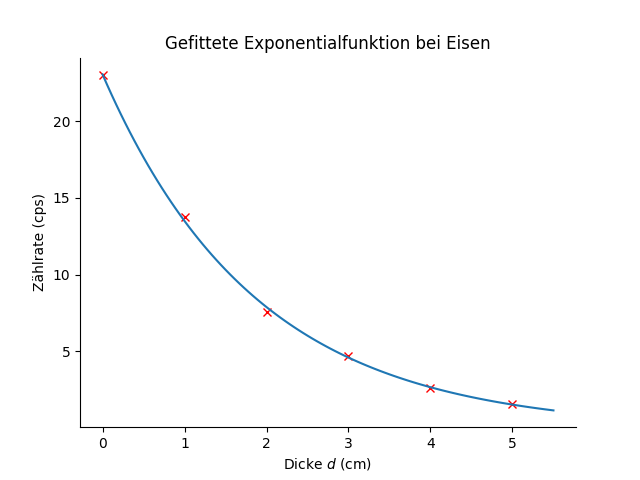
\includegraphics[width = 12cm]{Bilder/Auswertung/AbsorbtioskFe.png}
    \caption{Zählrate bei jeweiliger Absorberdicke $d$}
    \label{AbsorbtionkoeffFe}
\end{figure}

\begin{center}
    \centering
    \textcolor{red}{$\mu_{Fe}= (0,532 \pm 0,044) \mathrm{cm}^{-1}$}
\end{center}

\subsubsection*{Blei}

Bei diesem Teil könnte der Fehler zu klein abgeschätzt sein, da die verwendeten Bleiplatten in ihrer Dicke stark variiert haben. Daher kann es zu einem 
systematischen Fehler kommen, da die Anzahl der Absorberplättchen erfasst wurde, nicht aber die Gesamtdicke. Diese wurde einmal gemessen und mit der 
errechneten Dicke abgeglichen. Dabei wich diese um 50\% ab. Die kann unteranderem an Luft zwischen den nicht ebenen Plättchen liegen, aber auch an Dickeunterschieden.\\
Wie oben ist nochmal eine deutliche Zunahme des Absorptionsvermögens zu sehen. Dies liegt unteranderem an der höheren Dicht von Blei und dem höheren 
Wirkungsquerschnitt durch die höhere Kernladungszahl, welche sich in einem schnelleren Abfall des Kurve in Abbildung \ref{AbsorbtionkoeffPb} wiederspiegelt.

\begin{figure}[ht]
    \centering
    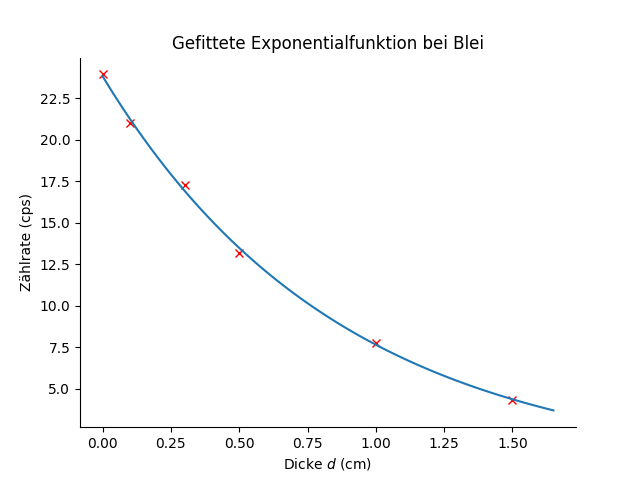
\includegraphics[width = 12cm]{Bilder/Auswertung/AbsorbtioskPb.png}
    \caption{Zählrate bei jeweiliger Absorberdicke $d$}
    \label{AbsorbtionkoeffPb}
\end{figure}

\begin{center}
    \centering
    \textcolor{red}{$\mu_{Pb}= (1.14 \pm 0.10) \mathrm{cm}^{-1}$}
\end{center}

\subsection{Massenabsorptionskoeffizient}

Der Massenabsorptionskoeffizient $\frac{\mu}{\rho}$ ist eine Größe, welche den linearen Absorptionskoeffizienten $\mu$ in Verbindung mit der Dichte $\rho$ des Materials setzt.
Man kann ihn also auch als Maß für den Wirkungsquerschnitt der Atome verstehen. Je größer der Massenabsorptionskoeffizient, desto wahrscheinlicher ist es für einen 
Nukleon von der Strahlung 'getroffen' zu werden. 

\begin{center}
    \centering
    \textcolor{red}{$\frac{\mu_{Al}}{\rho_{Al}} = (0,0727 \pm 0,0051) \mathrm{cm}^{2} \mathrm{g}^{-1}$}\\
    \textcolor{red}{$\frac{\mu_{Fe}}{\rho_{Fe}}= (0,0675 \pm 0,0055) \mathrm{cm}^{2} \mathrm{g}^{-1}$}\\
    \textcolor{red}{$\frac{\mu_{Pb}}{\rho_{Pb}}= (0,1011 \pm 0,0090) \mathrm{cm}^{2} \mathrm{g}^{-1}$}\\
\end{center}

Hierbei wurde für $\rho_{Al} = 	2,6989 \frac{\mathrm{g}}{\mathrm{cm}^3}$ \footnotemark 
\footnotetext{\url{https://de.wikipedia.org/wiki/Aluminium}, Stand: 16.09.2021 11:00}, $\rho_{Fe} = 	7,874 \frac{\mathrm{g}}{\mathrm{cm}^3}$ \footnotemark 
\footnotetext{\url{https://de.wikipedia.org/wiki/Eisen}, Stand: 16.09.2021 11:00} und
$\rho_{Pb} = 11,342 \frac{\mathrm{g}}{\mathrm{cm}^3}$ \footnotemark \footnotetext{\url{https://de.wikipedia.org/wiki/Blei}, Stand: 16.09.2021 11:00} verwendet.\\
Man sieht schön, dass der Wirkungsquerschnitt mit steigender Kernladungszahl stark ansteigt.


